\label{sec:background}

\newacronym{pow}{PoW}{Proof of Work}
\newacronym{pos}{PoS}{Proof of Stake}
\newacronym{edcc}{EDCC}{Executable Distributed Code Contract}
\newacronym{smr}{SMR}{State Machine Replication}
\newacronym{pbft}{PBFT}{Practical Byzantine Fault Tolerance}
\newacronym{tee}{TEE}{Trusted Execution Environment}
\newacronym{zkp}{ZKP}{Zero-Knowledge Proof}
\newacronym{dapp}{DApp}{Distributed Application}
\newacronym{dlt}{DLT}{Distributed Ledger Technology}
\newacronym{nft}{NFT}{Non-Fungible Token}
\newacronym{bose}{BoSE}{Blockchain-oriented Software Engineering}
\newacronym{ux}{UX}{User Experience}
\newacronym{abi}{ABI}{Application Binary Interface}
\newacronym{bpm}{BPM}{Business Process Management}
\newacronym{bpmn}{BPMN}{Business Process Model and Notation}
\newacronym{bp}{BP}{Business Process}
\newacronym{oop}{OOP}{Object-oriented Programming}
\newacronym{ccsm}{CCSM}{Consensus Controlled State Machine}
\newacronym{bpi}{BPI}{Baseline Protocol Implementation}
\newacronym{eea}{EEA}{Enterprise Ethereum Alliance}

The background chapter introduces fundamental concepts that are required throughout the rest of the work. This includes \gls{bpm}, \glspl{bct}, consensus algorithms, notations and blockchain-oriented software engineering approaches.

\section{Consensus}
\label{sec:background:consensus}
The upcoming section will give a small glimpse behind the concept of blockchains, it will introduce some consensus techniques for distributed computer systems, and explain the difference between specific leader-election mechanisms for blockchains such as \gls{pow} and \gls{pos}.


\subsection{Blockchain}
\label{sec:background:blockchain}
A blockchain is a linked list of records (so-called ``blocks''), where each record itself contains a list of transactions and the hash of the previous record originating from the so-called ``genesis block''. The links between records introduce unique properties such as immutability, transparency, and produces a traceable list that others can verify using cryptographic procedures. This creates an append-only data store that is typically distributed over a peer-to-peer network where each peer keeps a (full) copy of the history of transactions dispatched to the blockchain. In distributed environments, new blocks are typically determined and attached to the blockchain using consensus protocols that prevent Byzantine faults and establish trust. If blockchains are used in a financial context, they are sometimes referred to as \gls{dlt} as well~\cite{consensus_comparison_2019,security_patterns_in_ethereum}. Satoshi Nakamoto was the first to utilize them in a decentralized, trusted finance system in the form of Bitcoin. The core concept of Bitcoin is to provide a solution that solves the double-spending problem of virtual currencies and does not rely on a centralized, trusted third party~\cite{nakamoto2009}.


\subsection{Proof of Work (PoW)}
\label{sec:background:pow}
Bitcoin relies on \gls{pow} to elect a trusted proposer. Proposers are allowed to create new blocks (i.e.,\ a list of transactions and some metadata) based on the entirety of collected transactions so far. This block will then be distributed to the network using a form of total order broadcasting, a technique that ensures, that all participants receive the same blocks in the exact same order, and will be verified by other nodes that prevent double-spending attacks in case the proposer wants to abuse the fact of being trusted by others.

\gls{pow} is part of the Nakamoto consensus introduced in the Bitcoin whitepaper and is one of the many consensus techniques available. Miners compete on who is allowed to create the next block in the chain to earn (1) the right for coinbase transactions (the first transaction in a block that creates new units of said currency) and (2) the transaction fees. The more mining power a miner can utilize, the more often said miner will be elected as block proposer. Typically, Bitcoin aims to keep a block time of around 10 minutes (i.e.,\ it should take the entire pool of miners 10 minutes to mine a new block). This is achieved by dynamically adjusting the amount of work that has to be done depending on the network's total computing power. Therefore, the more computing power available, the harder the problem will become to solve (and vice versa in case miners leave the network). To be more formal, Nakamoto consensus (similar to Ethereum's consensus technique) wants miners to find a nonce $n$ such that

\begin{equation}
H(n || H(b)) < l
\end{equation}

where $l$ specifies the upper bound for the hash value produced by the hash of the previous block $b$ concatenated with the nonce. Once such an $n$ is found, other miners can easily validate the result. The algorithm adjusts the difficulty by adjusting how small $l$ is~\cite{consensus_comparison_2019}. This technique, however, became a target of certain controversy. The strong incentive of earning Bitcoins from mining new blocks leads to an uprise of miners in the network. The more miners, the harder the problem will become to solve. This increases the networks total energy consumption proportionally to the computational power available, causing the entirety of the Bitcoin ecosystem to consume approximately 99.27 TWh in the year 2022. To put this in perspective, the country of Austria will consume around 64.61 TWh in the same year according to predictions~\cite{cbeci}.

Another controversy regarding \gls{pow} in the context of Bitcoin is an attack vector called ``Selfish Mining'' that allows miners to earn disproportionately more revenue compared to their provided computational power. The idea behind this attack is to assume that miners will strategically collude in order to maximize the computing power to Bitcoins earned ratio. This is achieved by hiding successfully mined blocks from the main net, publishing them at certain times in the future, and thus wasting the computational power of trustful miners because the main net will always switch to the subchain that requires the most computational power (often referred to as the longest chain)~\cite{eyal2013}.


\subsection{Proof of Stake (PoS)}
\label{sec:background:pos}
\gls{pos} is one of the most popular alternatives to \gls{pow}. Even though it is similarly used as a leader-election mechanism, it does this in a much more energy-efficient way and thus overcomes one of the shortcomings of \gls{pow}. The idea behind this concept is that the more a node has at stake (be it in the form of an arbitrary resource), the more invested said one is to keep the system up and running correctly. This is achieved by choosing the next proposer based on the number of coins and the age of each coin. Nodes with a rather active wallet that contribute much to the network will thus be selected more often to propose a new block. If some node acts maliciously, the chances of being selected are reduced by the algorithm itself~\cite{consensus_comparison_2019}.

Even \gls{pos} comes with its quite unique downsides. One of those is the Nothing-at-Stake problem. It states that the validators (the equivalent in \gls{pos} to miners in \gls{pow}) of the network have an intrinsic financial incentive to participate in every fork of the network because doing so has no downsides but only increases the amount of reward a validator can collect. In practice, however, it is assumed that validators are aware that intentional network forking would raise doubts about the system itself, decreasing the coin's value. Each fork would live with a separate ledger containing different values for each participant, thus creating artificial inflation that further reduces the trust in the network. A reduced coin value will inevitably hurt the holders. Since (in \gls{pos}) the set of coin holders is exactly the set of participating nodes, it is intrinsic to the participant to prevent any value reduction and therefore does not perform Nothing-at-Stake attacks. Nonetheless, the Ethereum network introduced ``slashing'', a mechanism to destroy a certain percentage of the hostile participants stake, to further reduce the risk for such attacks~\cite{proof_of_stake}.



\subsection{State Machine Replication (SMR)}
\label{sec:background:blockchain:smr}
\gls{smr} is a concept at the heart of any distributed, fault-tolerant consensus system. First introduced by Leslie Lamport in~\cite{lamport1978}, given a set of rules, \gls{smr} ensures that each replica is in the same state after a message was sent from a client to perform some action. Those rules are as follows:

\begin{itemize}
\item Each non-faulty replica starts in state $s_0$
\item Each non-faulty replica that applies operation $o$ to state $s$ will end up in state $s'$
\item Each operation of each non-faulty client is executed
\item Each non-faulty replica executes the same order of operations $o_0, \ldots, o_i$
\end{itemize}

Each replica fulfills the first two properties without the need for any other distributed protocol. The latter two require some sort of total order broadcasting. Given that total order broadcasting can be reduced to the problem of consensus, some sort of distributed consensus protocol is required to establish a common order of operations~\cite{sousa12from_byzan_consen_bft_state_machin_replic}.



\subsection{Consensus Protocols}
\label{sec:background:blockchain:consensus-protocols}
A problem that emerged with distributed computer environments is achieving consistency in synchronous and asynchronous settings assuming that one or many nodes are faulty. This is known as the consensus problem of computer science.

Lamport et al.~\cite{lamport2002} exemplified this problem by using the metaphor of Byzantine generals\footnote{Lamports initial intention was to name this problem ``The Albanian Generals Problem''. In order to offend no readers, he was advised to use some no longer existing nationality like Byzantium, for example~\cite{kleppmann17desig}.} who have to decide on whether to attack or retreat in a battle. These generals, however, can only communicate with each other indirectly, causing delays and the possibility of messages getting lost. The authors have shown that at most $f$ generals are allowed to be traitors when there is a total of $n=3f+1$ generals on the field. If there are more than $f$ traitors, the consensus problem becomes undecidable. In computer networks, computing nodes, or processes, represent the generals. A node that, either intentionally or unintentionally, sends wrong messages to the other nodes or is holding them back is therefore Byzantine faulty.

However, one has to distinguish between Byzantine fault tolerance and crash tolerance. Byzantine faulty nodes typically cause more damage to the system than nodes that simply crash. To make a system crash tolerant, it is sufficient if the total number of nodes is $n=2f+1$. If $f$ nodes crash, the remaining $f+1$ nodes outnumber the crashed ones, and the system can still come to a consensus (assuming that Byzantine faulty nodes are no possibility in the given environment). Consensus protocols at least have to satisfy the following properties to be Byzantine or crash tolerant~\cite{sousa12from_byzan_consen_bft_state_machin_replic}:

\begin{itemize}
\item \textbf{Agreement}. Each non-faulty node must agree on the same value. They must not diverge; otherwise, the node is considered faulty.
\item \textbf{Integrity}. Each non-faulty node can only decide once (i.e.,\ once a value was decided, it is finalized and cannot be changed).
\item \textbf{Termination}. Each non-faulty node eventually makes a decision (i.e.,\ clients will get a response without the system getting stuck in an endless loop).
\end{itemize}

Additionally, to the properties above, some literature also adds the \textbf{Validity} property. Validity ensures that the value a node decides on was proposed by some other node. This rules out the trivial possibility that the deciding node always returns 0 (or some other predetermined constant) for any arbitrary input given.

Agreement, integrity, and validity are typical safety properties of a system, whereas termination is a liveness property~\cite{kleppmann17desig}.


\subsection{Synchronous vs.\ Asynchronous System Models}
Consensus literature distinguishes between synchronous and asynchronous system models and puts their work in either of both spotlights (or in both at the same time) to guarantee certain properties such as termination, for example.

The main difference between both is that synchronous systems proceed in a step-by-step manner. Those steps can be compared to moves in a chess game. Regardless of the time it took for each player to make a move, after each move, the chessboard is in a new and consistent state, and all participating parties (e.g.,\ the referee, the players, and the audience) are aware of said new state. In distributed computer systems, such steps are often modeled with time frames where timeouts enable the system to proceed to the next frame. Compared to synchronous systems, asynchronous systems do not need to satisfy timeliness properties. Algorithms modeled with asynchronous systems in mind are typically more general since they do not rely on the performance of the host system they are operated on. Since no communication is instantaneous, asynchronous system models typically reassemble the real world quite well. System models that have both synchronous and asynchronous properties are typically referred to as semi-synchronous or semi-asynchronous systems~\cite{aguilera2010,liskov1999,kleppmann17desig}.


\subsection{Public vs.\ Private}
From a philosophical point of view, consensus protocols and \glspl{dlt} can be classified into three distinct categories. Namely public, private, and consortium networks. Each of these has unique properties applicable to certain scenarios. Public \glspl{dlt}, for example, are usually favored in use cases where full decentralization and data integrity are desirable. The open consensus process allows anyone to validate the state of the \gls{dlt} at any given point in time and report erroneous states if necessary~\cite{consensus_comparison_2019}. Even though public \glspl{dlt} are highly decentralized in theory because participation is open to anybody, in practice, some degree of centralization may occur in the form of colluding miner pools nonetheless. This is something public \glspl{dlt} (such as Bitcoin and Ethereum) must consider to keep their system tamper-proof~\cite{nakamoto2009,buterin2020,eyal2013}.

On the other hand, private \glspl{dlt} are the complete opposite of public ones. Only authorized nodes are allowed to participate in the consensus process of the system. Some predetermined instances of a given organization will grant this permission to new participants. Even though read-only access could be granted to the public, private \glspl{dlt} typically choose not to, which gives a better sense of privacy. On the other hand, writing is entirely restricted to a pre-selected set of participants. This allows for finality because the number of participating nodes is well known but also makes the system prone to tamper attempts because trust is required in the organization that selects the participants~\cite{consensus_comparison_2019}.

Consortium \glspl{dlt} are \glspl{dlt} where multiple organizations (that might be in conflict of interest) come together to form a network that is partially decentralized and otherwise shares most of the properties of private ones. Which kind of \gls{dlt} and consensus protocol to choose from highly depends on the use case and who are the participants and organizations involved~\cite{consensus_comparison_2019}.


\subsection{Permissioned vs.\ Permissionless}
In consensus, the terms permissioned and permissionless refer to whether participation in a consensus protocol is restricted or unrestricted. Permissioned consensus requires a central authority (or a group of authorized participants) that can (1) authenticate each other as members of the group and (2) add new members. Permissioned consensus protocols that are publicly available can be a target for Sybil attacks\footnote{One entity pretends to be many.} and are therefore often replaced with permissionless consensus protocols (especially in the context of Blockchain technology). In contrast to permissioned consensus, permissionless consensus does not require any central authority. Bitcoin and Ethereum, for example, establish permissionless consensus through \gls{pow} and \gls{pos}. Sybil attacks are therefore ruled out by no longer relying on ``who you are'' but on ``what you have''~\cite{nakamoto2009,proof_of_stake}. Permissionless consensus is often favored in public networks, while permissioned consensus is favored in private networks allowing a subset of members to strictly control who is allowed to participate~\cite{consensus_comparison_2019}.


\subsection{FLP Impossibility Result}
\label{sec:background:flp}
Named after the authors (Fischer, Lynch, and Paterson), the FLP impossibility result shows that consensus becomes undecidable in a purely deterministic and asynchronous system if at least one node fails. Fischer et al.\ have been awarded with the Dijkstra prize for the significance of this result~\cite{impossibility_result_1985}.

According to the FLP theorem, all asynchronous consensus protocols have to decide on which two of the following three properties to guarantee~\cite{consensus_comparison_2019}

\begin{itemize}
\item \textbf{Safety}. When given the same input, all nodes should produce the same output (thus satisfying agreement, integrity, and validity).
\item \textbf{Liveness}. A client will eventually receive a response to its request (and thus satisfying the termination).
\item \textbf{Fault tolerance}. Even though not a must for consensus protocols, fault tolerance is still a property that is very much desirable. It allows a system to tolerate up to a certain number of faults $f$~\cite{liskov1999,tendermint2018,bessani14state_machin_replic_masses_bft_smart}.
\end{itemize}

In highly distributed environments (especially in Blockchain technologies), implementations cannot forfeit fault tolerance at any cost. The threat of nodes being faulty (or even malicious in the sense of Byzantine faults) leads the implementation to choose between the safety and the liveness property. \gls{pbft}, for example, strongly relies on the asynchronicity of safety and fault tolerance. In this case, the synchronicity of liveness is achieved by using timeouts and view changes and thus applying a step-by-step iteration as required in synchronous system models~\cite{liskov1999}.


\subsection{Tendermint}
Recent years led to a boom of new Byzantine fault tolerant system proposals in academia that suggest \gls{pos} as the ``better-suited'' alternative to \gls{pow} to overcome some of the mentioned shortcomings. The Tendermint consensus protocol (based on \gls{pbft}~\cite{liskov1999}), for example, suggests a purely deterministic and predictable algorithm based on who owns how much money to decide who is allowed to propose the next block. This kind of gossip protocol based on \gls{pos} reduces the overall electricity consumption and the system's complexity.

Similar to Bitcoin and Ethereum, Tendermint also relies on the strict assumption that less than $\frac{1}{3}$ of all nodes are Byzantine faulty (i.e.,\ produce wrong results or none at all either by accident or on purpose). Given that $n \geq 3f + 1$ is the minimum number of nodes, not more than $f$ nodes are allowed to be faulty. Otherwise, the Tendermint protocol cannot guarantee safety and liveliness properties for consensus~\cite{tendermint2018}.



\section{Blockchain-oriented Software Engineering}
With the growing interest in \glspl{dlt}, which allow users to run customized code in a distributed and trustless environment in the form of \glspl{edcc} as Ethereum does with smart contracts, systematic software development must be expanded upon in the context of blockchain technology~\cite{towards_blockchain_tactics}. Security, reliability, software architecture, and privacy are central aspects that must be considered when building applications using \glspl{dlt}~\cite{blockchain_oriented_software_engineering}.

Methodical software engineering is an applicable approach to these kinds of challenges. It is the engineering discipline that is concerned with all stages of building software products and the application of systematic engineering approaches to software development itself. Software engineering can be split into four distinct activities that are sometimes also referred to as the software process~\cite{software_engineering,swebok}:

\begin{itemize}
\item \textbf{Specification}. Together with the customers and users, software requirement engineers define constraints, functional and non-functional requirements that the resulting software product has to fulfill in order to achieve some business value.
\item \textbf{Development}. Software architects design the technical outline of the product given a certain specification, and developers implement this architecture using a set of requirements.
\item \textbf{Validation}. Software testers check if the product fulfills all specified requirements and therefore the customers and users needs. If this is not the case, the product is again modified according to the requirements.
\item \textbf{Evolution}. The finished product is further iterated upon to reflect the changing market and customer requirements.
\end{itemize}

The exact details of each software process step and the process itself depend on the specific use cases and the domain in which the product is being developed in (e.g.,\ the software process of an e-commerce and a spacecraft control system are most likely going to diverge)~\cite{software_engineering}.

When building software applications in the context of blockchain technologies, these process steps must be extended upon to deal with newly emerging challenges. Organizations focusing on blockchain-oriented software development will feel the urge to introduce new professional roles that fill the gap between business and financial aspects and technological expertise. Due to the strong focus on financials, security is also of utmost importance~\cite{blockchain_oriented_software_engineering}. \glspl{edcc} that malfunction may lead (and already have led) to tremendous losses. Hence, new formal methods must be devised that can be used to provide a profound tooling suite that is capable of analyzing, testing, and detecting programming errors in \glspl{edcc}. Especially the open source community has already developed some quite promising tools that are concerned with such issues. These tools are capable of performing static or dynamic byte or source code analysis to detect common security issues (examples of such are front-running, random numbers, or timestamp dependence), exploits, or formal guarantees. However, even more, and better tools that build upon existing open source technologies are expected to be developed in the future~\cite{tools_for_analyzing_smart_contracts}.

Creating specifications, documentation, or test plans for blockchain-oriented applications might require some modeling language to better visualize and understand certain problems. Therefore, \gls{bose} suggests to expand existing models such as UML into the domain of \glspl{dlt}. The newly created modeling language can then be further used to specify the software architecture. Besides defining a design notion, software architects will also be concerned with choosing which blockchain to use and how much blockchain truly is required for a certain use case (e.g.,\ it might be sufficient if only the hash values of some files are stored instead of storing the content of all files). Defining new macro-architecture design patterns for the definition and development process will also be of utmost importance. Some already existing patterns and design approaches are discussed in the sections below~\cite{blockchain_oriented_software_engineering,how_much_blockchain_do_you_need}.


\subsection{Hybrid App Design}
Complex software applications typically consist of multiple loosely coupled components that each strive for high cohesion. A more informal definition for this circumstance would be ``what changes together, stays together''~\cite{newman2019_monolith_to_microservices_constantines_law}. These properties allow each component to be reused through standardized APIs and maintained without affecting other components, therefore keeping change concentrated in a single spot. Following the low coupling high cohesion principle, new software engineering approaches, in particular \textit{Chaos Engineering}\footnote{Initially developed by Netflix to provide system resiliency}~\cite{chaos_engineering}, emerged in the industry that have been quickly adapted by others. Other principles such as \textit{Acyclic Dependencies} and \textit{Reuse Release Equivalence} are also rather common when talking about software application decomposition and domain-driven design in modern software architecture~\cite{clean_architecture}.

Building upon mentioned principles, a new approach was derived specifically for creating hybrid applications where only certain components must communicate with the blockchain directly. To achieve this goal, Florian Blum et al.~\cite{how_much_blockchain_do_you_need} suggest a three-step process to identify specific properties that are later used to derive the system architecture:

\begin{enumerate}
  \item \textbf{Identify participants}. Defines the boundaries for a specific use case (and in parts for the system itself) by identifying relevant actors (e.g.,\ ``contractor'' or ``supervisor'').
  \item \textbf{Identify trust relations}. Defines in what kind of trust relationship actors stand to each other. Trust relations range from low trust classes (e.g.,\ ``trust in unknown persons'') to high trust classes (e.g.,\ ``trust in the company one is employed at'') and might be uni- or bidirectional.
  \item \textbf{Identify interactions}. Defines which actors interact with each other and modify shared data. This step might look quite similar to the previous one, but actors that interact with each other might not have to trust each other and vice versa.
\end{enumerate}

In the last step, the system architecture can be derived when all properties are eventually identified. Precisely, the question is answered if blockchain technology is required in the first place and, if so, where and how. Certain actors might already be in a mutual trust relationship that nullifies the advantages of trustless and tamper-proof environments. Adding blockchain technology would thus solely increase development overhead. Other actors, however, might be in somewhat brittle trust relationships that require frequent interactions nonetheless. Communication over the blockchain could be advised.

The third possibility are transitive trust relations. Let $T$ be the homogeneous relation between two participants in set $P$ where trust is established either mutually or by using blockchain-based technologies. Then, participants $a$ and $c$ are in an implicit transitive trust relation if $a$ trusts $b$ and $b$ trusts $c$. This circumstance is formally expressed in first-order logic:

\begin{equation}
\forall a,b,c \in P : (aTb \land bTc) \implies aTc
\end{equation}

Those kinds of relations build the transition points from blockchain-based trustless environments ($bTc$) to environments with mutual trust properties (such as $aTb$ w.l.o.g.) using the mediator participant $b$~\cite{how_much_blockchain_do_you_need}. However, which specific kind of blockchain technology (public vs.\ private or permissioned vs.\ permissionless, for example) to use and where to employ them highly depends on the domain-specific use cases. Thus, users of the framework should orient themselves towards the goals that stakeholders wish to achieve with the software product (i.e.,\ keep business strategies in mind) and use them to derive architectural tactics using the described process~\cite{building_hybrid_dapps_using_blockchain_tactics}. It is only a first step towards systematic blockchain-oriented software engineering, but already models an intuitive way of deriving a macro-architectural draft for hybrid apps.


\subsection{Transactional Patterns}
Distributed applications as part of hybrid architectures typically consist of two components: The business logic and the frontend facing the user. The communication between those two components can be modeled in different ways where each introduces certain advantages and disadvantages in either \gls{ux} or trust. The goal of design patterns, in general, is to provide some (adjustable) solution to non-trivial recurring problems in software design that eventually lead to positive effects, especially regarding non-functional requirements~\cite{design_patterns,security_patterns_in_ethereum}. Transactional patterns are design patterns in the context of \glspl{dlt} concerned with the communication between the frontend and the blockchain, who verifies transactions, and who pays the transaction fees~\cite{engineering_software_architectures_of_BO_Apps}.

One common pattern in open source software are the so-called \textit{Self-Generated Transactions}. Users interact directly with the blockchain and the desired \gls{edcc}. This is achieved in either of three ways: (1) sending transactions without detours to some blockchain node (e.g.,\ by using the geth client\footnote{\url{https://geth.ethereum.org/} (accessed on 2022-11-29)}), (2) using some low-level wallet web frontend (e.g.,\ MyEtherWallet\footnote{\url{https://myetherwallet.com/} (accessed on 2022-11-29)}) or (3) by using browsers with built-in wallets. This approach requires little to no trust in any abstract system, but requires users to have at least some technical knowledge (especially because this approach is quite error-prone). Furthermore, \glspl{abi} must be publicly available. Self-generated transactions are thus quite useful for testing \glspl{edcc} during development~\cite{engineering_software_architectures_of_BO_Apps}

\textit{Self-Confirmed Transactions} are an alternative to self-generated transactions. Instead of the users creating the transactions themselves, the frontend application generates them. This requires some trust towards the distributed app, but it is more convenient since users only have to take care of their private key~\cite{engineering_software_architectures_of_BO_Apps}. The third pattern are \textit{Delegated Transactions}. Users interact with the frontend without even noticing the usage of blockchains as data storage in the backend. Frontends use an arbitrary technology to communicate with the backend (e.g.,\ REST or gRPC). The backend can then perform off-chain computations and batch update the blockchain state if necessary. This allows for further cost optimizations (because expensive storage and computation can be performed off the blockchain) and does not require users to keep their own wallet~\cite{eberhardt17off_block}. An extension to delegated transactions offers the \textit{Meta Transactions} pattern. Users can still sign transactions with their private keys if necessary without the need for private wallets. This allows for tracking transactions and offers extended transparency. Both delegated and meta transactions undoubtedly offer the best \gls{ux} but require a substantial amount of trust in the established infrastructure beforehand. Which transaction technique to use once again highly depends on the use cases, stakeholder requirements, and the target audience of the system~\cite{building_hybrid_dapps_using_blockchain_tactics}.



\section{Onchain vs Offchain}
Blockchains such as Bitcoin and Ethereum aim to transfer value in an environment that does not rely on any centralized trusted third party. This kind of decentralization is achieved by establishing a peer-to-peer network in which each node is a full replication of the entire state of the system, guaranteeing, due to the intrinsic property that each node is incentivized in some form to act trustworthy, that nodes validate one another regularly and punish malicious behavior. In such an environment, however, transactions must be executed on all peer nodes of the network equally. Blockchains that allow custom code to be executed in the form of smart contracts must accommodate the additional execution and storage requirements in some form. Ethereum, for example, associates each operation with a fixed cost, which makes on-chain execution of more complex programs also more expensive~\cite{buterin2020}.

The limited (and costly) on-chain storage furthermore does not allow developers to store large files like images or videos directly on the blockchain since the cost would be unproportionally high. Blockchains also do not accommodate for any privacy concerns. Any information (even in the form of private variables in smart contracts) can easily be accessed by any participant. Hence, the need for off-chaining storage and computation solutions (sometimes referred to as \textit{blockchain tactics}) was born~\cite{towards_blockchain_tactics,eberhardt17off_block}.


\subsection{Smart Contracts}
Some blockchain implementations allow developers to write custom applications that are executed enclosed by their trustless and tamper-proof environment. Those applications are typically referred to as smart contracts or \glspl{edcc}. Ethereum was one of the first technologies that provided a Turing-complete and tamper-proof programming language by leveraging on their virtual machine with Solidity\footnote{\url{https://soliditylang.org/} (accessed on 2022-11-29)} as their syntax.

Smart contracts\footnote{Not to confuse with legal contracts.}, however, are limited in their capabilities because they must be deterministic and return the same results on every node of the network that executes the code. This means that reading from HTTP sockets or a local file system, for example, is out of scope. Even the task of producing pseudo-random numbers is a non-trivial challenge in Solidity and has to be implemented with caution, otherwise causing severe security issues. Allowing such operations would immediately render consensus undecidable since every node might produce another output for the same input and sequence of instructions executed (one node times out on the network connection, while another computes the result as expected, for example)~\cite{buterin2020}.


\subsection{Offchaining Storage}
\label{sec:background:on_vs_off_chain:offchaining_storage}
Blockchains are typically maintained by a larger number of nodes where each node acts as a replication that holds a copy of the chain's current and previous state. This allows all actors to perform operations in a trustless environment but comes at the cost of information being redundantly stored on each node. Hence, a file with $N$ bytes grows linear with the number of nodes. On a chain with $M$ nodes, a total of $N \cdot M$ bytes of disc space is required. Besides being expensive, data on the blockchain is also publicly available to anyone at any time~\cite{nakamoto2009,buterin2020}.

One might conclude that storing a reference to a large data set which itself is stored on a cloud-native storage solution like Amazons S3\footnote{\url{https://aws.amazon.com/s3/} (accessed on 2022-11-29)} or Google Cloud Storage\footnote{\url{https://cloud.google.com/storage} (accessed on 2022-11-29)} might be sufficient. Doing so, however, would allow users to change the data in the cloud, whereas the reference in the blockchain stays the same. This might be a good approach if trust is not of utmost importance for the participants using the data like, for example, for the images used by the online platform for the CryptoKitties\footnote{\url{https://cryptokitties.co/} (accessed on 2022-11-29)} \gls{nft}. In cases where participants are in a conflict of interest and rely on a blockchain's trustless and tamper-proof environment, this naive approach is no longer viable. Thus, one has to find a solution that is manipulation resistant if storage of large amounts of data is required~\cite{how_much_blockchain_do_you_need,eberhardt17off_block,weber2019_architecture_for_dapps_blockchain_patterns}.

One way to achieve manipulation resistance in off-chain storage solutions is to make stored data immutable (i.e.,\ neither allowing manipulation nor deletion). However, this must be enforced by the off-chain storage itself. Another, more convenient way is to use the \textit{Content-Addressable Storage Pattern} as proposed by Eberhardt et al.~\cite{eberhardt17off_block}. This pattern aims to provide a solution that allows trustless outsourcing of large amounts of data. This is achieved using so-called content-addressable storage in conjunction with a smart contract. A content-addressable storage is a storage solution that references all its data by a unique address derived from the hash value. Thus, if the content $C$ of some file $F$ has been modified, a new address from $H(C)$ will be derived (given practical collision resistance). A smart contract can now use $H(C)$ to reference the immutable file $F$ and validate if $F$ has changed in a cost-efficient way either off- or on-chain. Off-chain storage solutions must be highly available; otherwise, the system sacrifices its termination property in the long run. Implementations of content-addressable storage solutions that are available and durable are for example the Interplanetary File System~\cite{interplanetary_file_system} and Swarm\footnote{\url{https://ethersphere.github.io/swarm-home/} (accessed on 2022-11-29)}.


\subsection{Offchaining Computation}
\label{sec:background:on_vs_off_chain:offchaining_computation}
Performing computation on blockchains is similarly expensive as storing data. Blockchains that support \glspl{edcc}, as Ethereum does in the form of smart contracts, typically associate a fixed fee to each operation performed in such a contract. Even the most trivial operations such as multiplications or divisions come at some cost (i.e.,\ one pays money to operate a smart contract)~\cite{ethereum_yellow_paper}. Data that one has to operate on might be private and only available to a single user. This is an inherent problem of blockchains since all the information has to be publicly available to anyone at any time to perform deterministic computations on all nodes respectively. Naive off-chaining approaches, however, will introduce trust problems. The result from the off-chain computation might be faulty, or off-chain systems might send wrong computation results to gain an advantage. Careful consideration of these possibilities is advised, and verification is required (which is the minimum amount of computation that has to be performed on-chain to assure trust)~\cite{eberhardt18off_model_approac_off_comput}.

One way to preserve the trustlessness property of blockchains in off-chain computations is the \textit{Challenge Response Pattern}. First proposed by Eberhardt et al.~\cite{eberhardt17off_block}, this pattern aims to perform expensive computations off-chain while state transitions are validated on-chain. One participant will generate a challenge transaction of some off-chain computation (imagine checking the win conditions for a chess game). Other participants are thereafter incentivized to check if the given challenge is indeed a valid claim. If so, no further transactions must be sent to the blockchain. Some timeout (required to fulfill the termination property) will trigger the on-chain state transition. Thus smart contracts must not rely on on-chain checks themselves. The state transition is canceled if participants send a valid response in time. The layer-2 rollup \textit{Optimism}\footnote{\url{https://optimism.io/} (accessed on 2022-11-29)} leverages upon this pattern for example.

The \textit{Off-chain Signatures Pattern} offers an alternative where state transition is performed off-chain and implicitly agreed upon by all participants using their unique signatures. The only purpose of smart contracts in this pattern is to validate the signatures, check if all participants have signed a given transaction, and perform an immediate state change derived directly from the new state information in the transaction. The off-chain signatures pattern thus allows participants to perform as many off-chain peer-to-peer transactions as required without the involvement of the blockchain itself. A state-changing transaction is sent to the smart contract if all participants agree upon the new state. Compared to the challenge response pattern, this pattern requires less blockchain transactions overall, thus leading to a significant cost reduction. However, one has to consider a certain loss of traceability since more transactions are performed off-chain than on-chain~\cite{eberhardt17off_block, eberhardt18off_model_approac_off_comput}. Some implementations of this pattern already exist to cope with the low throughput of modern blockchain technologies~\cite{taxonomy_of_blockchain_based_systems}. These include state channel implementations such as the Perun\footnote{\url{https://perun.network/} (accessed on 2022-11-29)} or the Raiden\footnote{\url{https://raiden.network/} (accessed on 2022-11-29)} network.


\subsection{Offchaining Trust}
\label{sec:background:on_vs_off_chain:offchaining_trust}
Other techniques have been proposed to cope with the privacy issues of blockchains in a similar fashion. Hybrid \glspl{dapp} that only partially rely on blockchains depending on the level of trust required for each stakeholder can reduce the amount of transactions required~\cite{how_much_blockchain_do_you_need}. Enclave-based off-chain computing is another approach that utilizes \glspl{tee} to perform computations in a fully trusted environment that guarantees source code confidentiality and execution integrity. First defined by the OMTP~\cite{omtp09_tee_spec} in 2009, primarily for use in mobile devices, they quickly became a promising technology for edge computing and the \gls{iot}. Enclave-based computing also allows the usage of confidential information without making it publicly available to the entire blockchain network~\cite{fu21_tee_for_iot}.

As a promising alternative to \glspl{tee}, privacy concerns can be tackled by leveraging on \glspl{zkp}. This cryptographic technique allows participants to prove to some third party that they know a specific value $D$ without revealing $D$. The level of confidence that the participants possess this kind of knowledge is comparable to the confidence hash algorithms provide when showing that a specific piece of information produces a particular hash value. In the context of blockchains, \glspl{zkp} can be used to prove that off-chain computations have been performed according to a certain specification without revealing the computation logic itself or to prove that a participant possesses some confidential information without revealing it, for example. In order to generate \glspl{zkp}, a zero-knowledge circuit is required, which implementation is very much use case specific. The generation of such proofs is computationally rather expensive, but verifying their correctness, on the other hand, is not~\cite{sun2021_survey_of_zkp_on_blockchain}.

A third technology that allows participants to ensure trust to some extent without revealing confidential information is \textit{Homomorphic Encryption}. Homomorphic encryption allows for computation to be performed on encrypted data. Such a system is formally defined as $\xi(x) \odot \xi(y) = \xi(x \odot y)$ where $\xi$ is the encryption function, and $\odot$ is an arbitrary operation in this homomorphic system. One possible scenario for homomorphic encryption is that a piece of information $z$ is encrypted by participant A. Participant B then performs an operation upon the encrypted piece of information $\xi(z)$ resulting in $\xi(\bar{z})$ and participant $A$ then extracts $\bar{z}$ by decryption~\cite{jayabal20_blockchain_centered_homomorphic_encryption}. Depending on the specifics of the computational problem, some of the mentioned alternatives might even be combined~\cite{eberhardt18off_model_approac_off_comput}.


\subsection{Keeping a small footprint}
\label{sec:background:on_vs_off_chain:pattern_small_footprint}
Blockchain transactions are expensive operations. Developers should therefore minimize the number of transactions to reduce the overall cost of their application. One option to do so regarding smart contracts is to check the validity of state transitions off-chain and only trigger an on-chain validity check if the off-chain one fails. Of course, such an approach would require other techniques to guarantee trust, such as the \textit{Off-chain Signatures Pattern} or the \textit{Delegated Computation Pattern}. Another option to reduce cost is to reduce the amount of storage required in smart contracts and to optimize for writes instead of reads. This might look counter-intuitive to some developers because it increases the amount of computations performed. However, this approach will move the computation from the expensive blockchain nodes to cheap off-chain systems. In other words: one should not store redundant information but compute derived information locally. This is only possible because reading from the blockchain is feeless compared to writing. These general guidelines are known as \textit{Low Contract Footprint Pattern}~\cite{eberhardt17off_block}.


\section{Business Process Management}
\label{sec:background:bpm}
In recent years, \gls{bpm} has received more and more attention from both the industrial and computer science communities because it can not only be used to improve business operations and decrease production costs, but it also gives an overview of the broader requirements that a software system has to fulfill and therefore allows better planning to improve scalability and robustness even considering the integration of blockchain as a reliable source of truth. By definition, \gls{bpm} assumes that every product a company might produce is the result of a series of well-defined activities\footnote{Later on also referred to as ``tasks''.} that are performed in sequence or in parallel; ordering, structuring, and optimizing these activities according to the needs of the company is one of the key concerns of \gls{bpm}. This is achieved by the concepts and methodologies that \gls{bpm} provides to support the design and analysis of activities. The resulting series of activities, jointly implementing a business goal, is called a \gls{bp}. \glspl{bp} typically encapsulate activities that are only performed by a single company or organization. However, interactions with activities that are performed by others are not prohibited and, in certain scenarios, even desirable, as inter-organizational business process management shows~\cite{weske2012_bpm_introduction}. One might consider the role of a construction company instructed to refurbish the park in the city center as an example of a \gls{bp} that relies on external activities. The construction company has to gather information about the surrounding environment (historical and protected land sites, water pipes, and electrical infrastructure running underneath or beside the existing park, etc.) from the city council, has to contract city planners to design the new park and has to get in contact with suppliers that deliver required resources on-time. Another example worth mentioning might be a building administrator (responsible for large commercial or residential buildings) who has to contract maintainers for critical facilities like elevators or escalators. Organizing these kinds of activities in a timely and cost-optimized fashion is a typical use case for \gls{bpm} and shows the need for activities that interact and depend on the activities of other companies, suppliers, and organizations. The upcoming sections introduce notations that are used to create sound models of such \glspl{bp} and inter-organizational \glspl{bp} in the form of orchestrations and choreographies that already integrate core concepts for software systems like data dependencies between activities and object life-cycles in artifact-centric \gls{bpm}\footnote{\gls{bpm} that evolves around the resulting product and the produced artifacts of each activity and sub-process instead of the entire series of activities. This approach might be beneficial when \glspl{bp} are integrated into classical object-oriented software architectures due to the similarities of life-cycles of objects in \gls{oop} and real-world objects~\cite{data_driven_choreography_data_reusability_lichtenstein,modeling_blockchain_based_choreographies}.}~\cite{weske2012_bpm_properties_of_business_processes}.% Due to the level of abstraction these notations provide in being entirely technology agnostic, they are also used later on to describe use cases that are (partially) rely on the blockchain.


\subsection{Business Process Model and Notation}
\label{sec:background:bpm:bpmn}
The \gls{bpmn} is a graphical specification language for business process modeling maintained by the Object Management Group (OMG). It consists of well-defined elements with very specific purposes such as~\cite{bpmn_v2_spec,omg2010_bpmn_by_example}:

\begin{itemize}
    \item \textbf{Flow objects}. Activities and events to be performed during the course of a \gls{bp}. This includes gateways that allow parallel process execution and exclusive process execution.
    \item \textbf{Connecting objects}. Linking flow objects together to indicate transitions from one object (e.g.,\ a gateway) to another object (e.g.,\ an activity). \textit{Connecting objects} also allow associating messages or notes to flow objects.
    \item \textbf{Swim lanes}. Grouping together coherent flow objects and connecting objects. Swim lanes are typically used to depict companies, organizations, or departments in inter-organizational \glspl{bp}.
\end{itemize}

The upcoming paragraphs introduce more complex notations of \gls{bpmn} by example, by building upon the aforementioned \gls{bp} of a building administrator contracting a maintenance service. This exemplary \gls{bp} is a simplification of a real-world scenario and was derived from a model created with domain experts. Figure~\ref{fig:background:maintenance_contractor_only} shows the simplified workflow of the facility maintainer. Maintenance is only started upon receiving the \textit{message start event} ``receive maintenance request''. Afterwards, the maintenance is performed, completed and, if accepted by the supervisor, an invoice together with a maintenance report forwarded to all required parties.

\begin{figure}[h]
    \makebox[\textwidth][c]{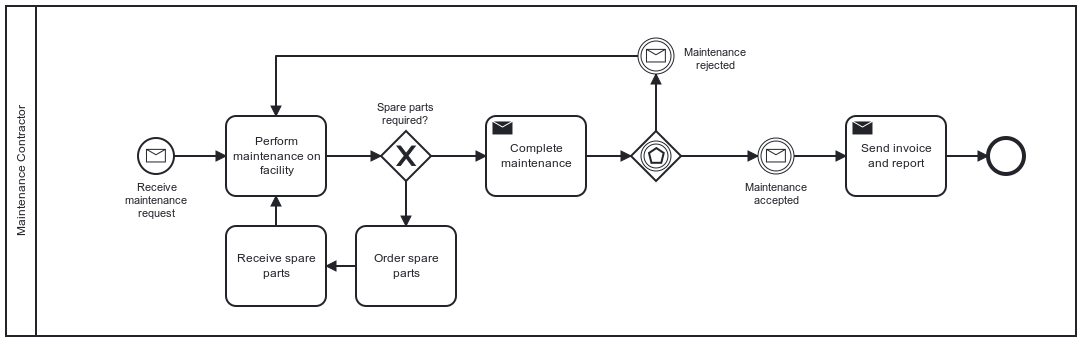
\includegraphics[width=1\textwidth]{background/graphics/maintenance-contractor-only.png}}
    \caption{A simplified business process of a maintenance contractor.}
    \label{fig:background:maintenance_contractor_only}
\end{figure}

This \gls{bpmn} diagram also makes use of some gateways. After the maintainer has performed her first maintenance cycle on the facility, she has to report if any spare parts are required to complete maintenance. If so, spare parts will be ordered; otherwise, the maintenance is complete. For constructs like these, \gls{bpmn} introduces the so-called \textit{exclusive} gateway that only allows execution of one of the subsequent activities. In other words, either the spare parts must have been ordered, received, and replaced in the facilities before maintenance can be completed, or no spare parts are required at all. After maintenance has been completed by the maintainer and thus the maintenance contractor, a third party (in this example, the building administrator) can either accept or reject the maintenance. Waiting for activities of third parties to complete is achieved with the \textit{event-based} gateway. This gateway halts further process execution until one of the subsequent events occurs~\cite{weske2012_bpm_introduction,omg2010_bpmn_by_example}. Single-party \gls{bpmn} diagrams like these are rarely useful because they do not highlight interactions with third parties and, thus, possible conflicts of interest. Introducing a customer as a building administrator into the diagram in figure~\ref{fig:background:maintenance_contractor_only} will improve the example and shows how interactions occur in certain situations. Figure~\ref{fig:background:maintenance_full}\footnote{Created with \url{https://bpmn.io/} (accessed on 2022-11-01)} depicts the full building administrator use case from section~\ref{sec:background:bpm}.

\begin{figure}[h]
    \makebox[\textwidth][c]{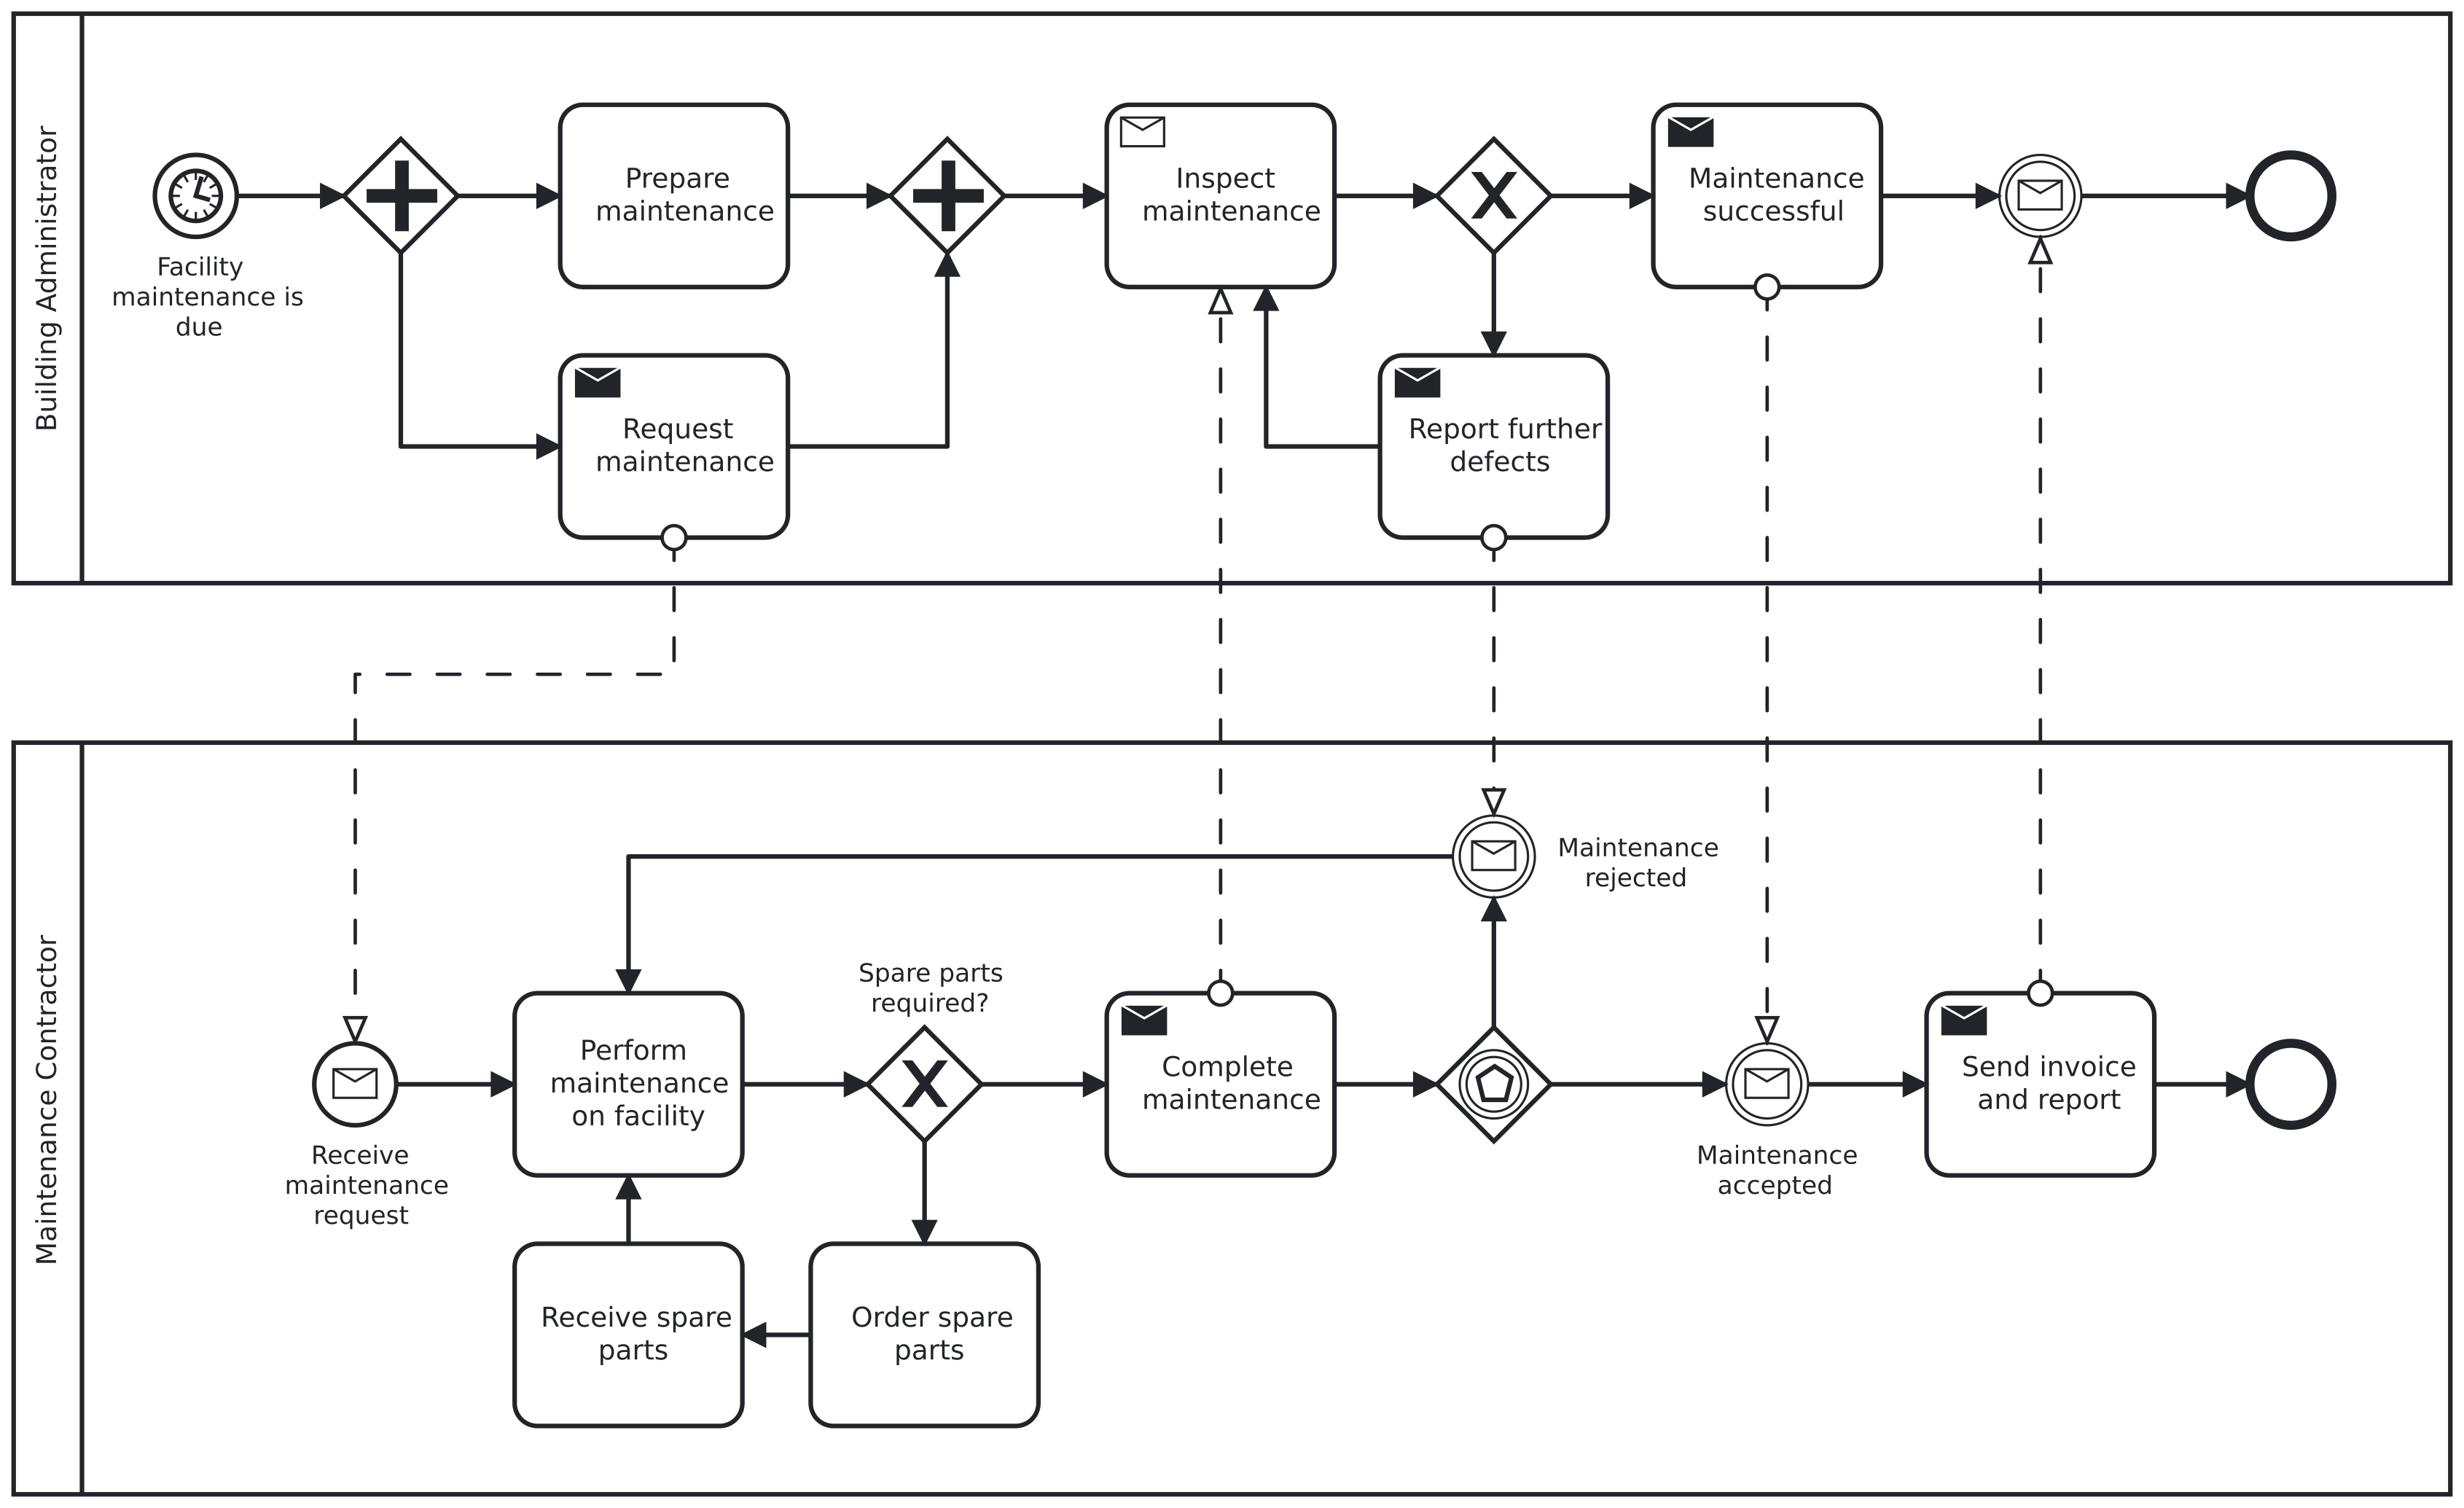
\includegraphics[width=1\textwidth]{background/graphics/maintenance-full.png}}
    \caption{More complex two-lane diagram with interactions between participants.}
    \label{fig:background:maintenance_full}
\end{figure}

The facility maintenance workflow on the side of the building administrator is triggered by the \textit{timer start event} ``facility maintenance is due''. This kind of event indicates that a \gls{bp} should be started whenever the time constraints associated with the event are met. These might be abstract, as depicted in figure~\ref{fig:background:maintenance_full}, or discrete in the form of a timely interval or any other time constraint. When maintenance is triggered, the responsible building administrator has to get in contact with the maintenance contractor and, at the same time, prepares the facility and the building for the upcoming maintenance and notifies staff and local residents (e.g.,\ by sending a notice that the elevator is not available until maintenance is complete). Parallelization of activities in \gls{bpmn} is achieved by employing so-called \textit{parallel} or \textit{split} gateways. A \textit{join} gateway is used afterwards to merge all concurrent branches back together if they have been successfully completed. When maintenance is done, the building administrator inspects the maintainer's work and either certifies the maintenance or reports further defects. Once again, this is achieved by employing the \textit{exclusive} gateway of the \gls{bpmn} notation~\cite{bpmn_v2_spec,weske2012_bpm_introduction}.

% As mentioned before, this example is a greatly simplified \gls{bp} that was derived from real-world \glspl{bp} used by domain experts to visualize some of the concepts introduced by \gls{bpmn}. However, \gls{bpmn} has proven itself as a valuable tool in computer science and business administrations due to its ubiquitous, unambiguous, and well-defined elements. Thus, the remainder of this work also makes use of \gls{bpmn} to introduce and describe other use cases as well.


\subsection{Orchestration and Choreography}
\gls{bpmn} introduces a specification language that allows its users to define \glspl{bp} on a rather granular level using flow and connecting objects. Typically, these objects are grouped into swim lanes where each swim lane defines a single party (e.g.,\ a company or organization). The business process defined for this party is also referred to as \textit{orchestration} or \textit{process orchestration}~\cite{bpmn_v2_spec}. Orchestrations are used to provide a more detailed view of activities (and their associated execution constraints) that interact with both external and internal activities~\cite{orchestration_and_choreography,weske2012_bpm_process_orchestration}. While orchestrations focus on one party's perspective, \textit{choreographies} focus on coordinating interactions between multiple parties. Choreography diagrams that depict a sequence of messages exchanged between parties typically represent a distributed process and activity flow. In other words, the interactions between different orchestrations can be formalized as choreography~\cite{trust_in_service_oriented_ds_through_blockchain,weske2012_bpm_process_choreographies}. Choreography diagrams are especially useful in business-to-business scenarios where activities of one business have to interact and exchange messages with activities from other businesses~\cite{orchestration_and_choreography}. Due to the fact that choreography diagrams are part of the \gls{bpmn} specification, their notations are also quite similar~\cite{bpmn_v2_spec}. Instead of describing activities, choreography diagrams focus on so-called \textit{choreography tasks}. Each choreography task represents the interaction between two or more parties. These tasks are connected with each other by reusing \gls{bpmn} \textit{connecting objects}. The building administrator and maintenance contractor example is depicted as choreography diagram in figure~\ref{fig:background:maintenance_full_choreography}.

\begin{figure}[h]
    \makebox[\textwidth][c]{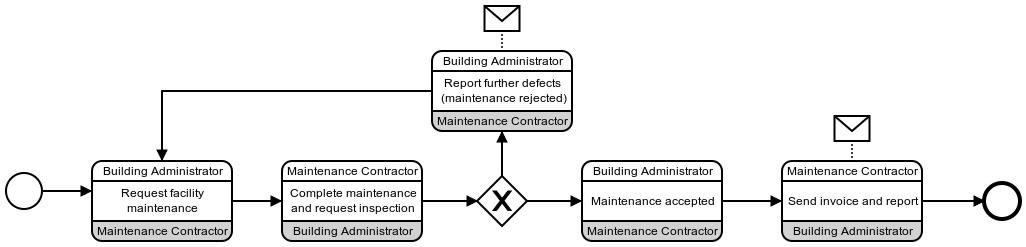
\includegraphics[width=1\textwidth]{background/graphics/maintenance-full-choreography.png}}
    \caption{Choreography diagram highlighting interactions between two participants.}
    \label{fig:background:maintenance_full_choreography}
\end{figure}

Graphically, choreography tasks are denoted with boxes with rounded corners. The inside of the box describes the message exchanged, and two bands, one at the top and one at the bottom of the box, represent the involved parties. The band of the initiating party typically uses the same color as the box itself, whereas the darker band is dedicated to the receiving party. Letter-like symbols connected to the bands of the parties attach supplementary information to the message~\cite{trust_in_service_oriented_ds_through_blockchain,bpmn_v2_spec}. In this example, an invoice and report are added to the last choreography task before reaching the \textit{end event}.

% Besides \gls{bpmn} diagrams, later sections of this work also make use of choreography diagrams to better visualize message exchanges between counterparties and even the blockchain itself.



\section{Baseline Protocol}
\label{sec:background:baseline_protocol}
The Baseline Protocol, a recently defined \gls{eea} standard and OASIS open source project, tries to enable businesses and organizations to synchronize complex \glspl{bp} as well as associated data and messages and increase overall system resiliency. The \gls{bp} introduced in section~\ref{sec:background:bpm:bpmn} is only a simplification of a far more sophisticated scenario. Synchronizing state between counterparties is, therefore, inevitably more difficult than expected. The Baseline Protocol aims to solve this issue by leveraging on the blockchain (or other forms of shared state machines) as an immutable and traceable source of truth that involved participants can trust. Over time, this can increase information security and operational integrity because systems of record no longer have to share potentially confidential data or internal business processes but rely on profound proofs that specific properties of \glspl{bp} have been fulfilled~\cite{baseline_spec}. The standard, however, is still in a volatile state and can introduce breaking changes at any time. Therefore, the upcoming sections only give a rather broad overview of its concepts.


\subsection{Architecture and State Synchronization}
\label{sec:background:baseline_protocol:architecture}
To ensure ``workflow integrity, event ordering, and data consistency'', the Baseline Protocol specifies that a compliant implementation must rely on a \gls{ccsm}. Blockchains like Ethereum and Bitcoin are implementations of such. The systems of record that the \gls{bpi} communicates with are only loosely coupled with the \gls{bpi} itself in the form of a standardized API~\cite{baseline_spec}. Figure~\ref{fig:background:maintenance_multiple_participants} shows a software architecture with a \gls{bpi} integration.

\begin{figure}[h]
    \makebox[\textwidth][c]{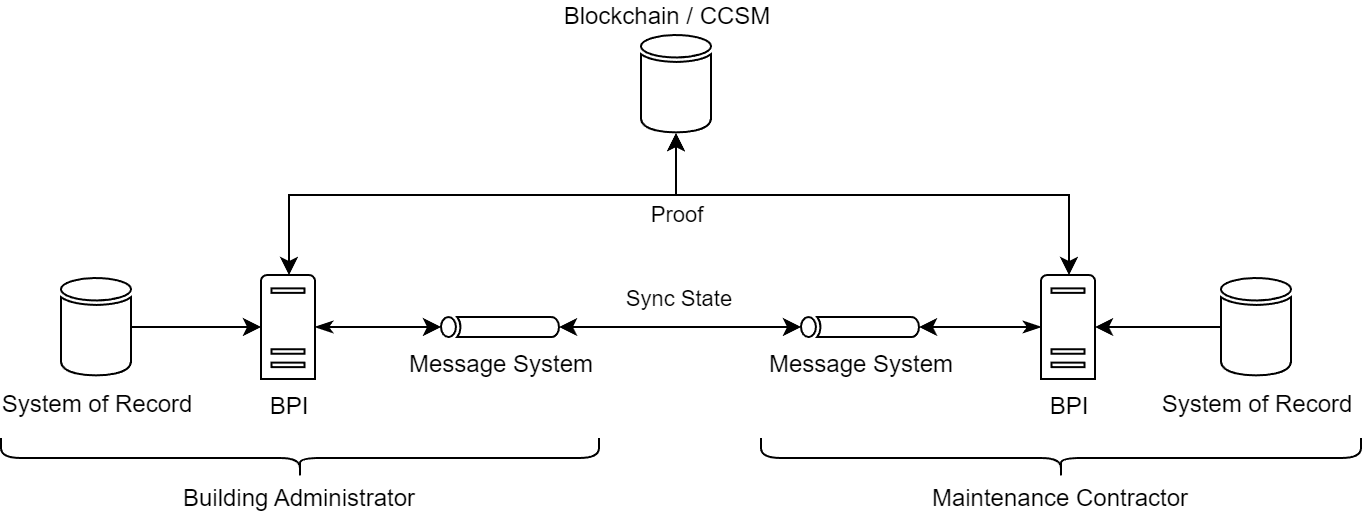
\includegraphics[width=.95\textwidth]{background/graphics/maintenance-baseline-architecture.drawio.png}}
    \caption{Integration of a \gls{bpi} into the two-party facility maintenance system.}
    \label{fig:background:maintenance_multiple_participants}
\end{figure}

All involved participants (the building administrator and the maintenance contractor) keep their own system of record that contains the current state of the workflow, required documents, or even confidential data that is not allowed to leave the organization's network. Communication between participants is solely handled by the \gls{bpi} to exchange necessary information. The \gls{bpi} generates a proof that the document to be exchanged follows the service-level agreements and stores it on a \gls{ccsm} to acquire properties such as traceability, immutability, workflow integrity, or data consistency. On the other hand, the data is transmitted entirely off-chain to keep the smallest footprint possible and reduce transaction cost. This ensures that confidential data can be kept private if necessary and allows sending large amounts of data to counterparties without breaking the blockchains' block size limit. Figure~\ref{fig:background:maintenance_report_baseline} gives a more in-depth explanation of how communication between counterparties can be realized according to the standard and shows the Baseline Protocol compliant process of the maintenance contractor sending the maintenance report to the building administrator in the form of a flow chart. A system of record that wants to take advantage of the properties of the Baseline Protocol at least has to implement the depicted communication.

\begin{figure}[h]
    \makebox[\textwidth][c]{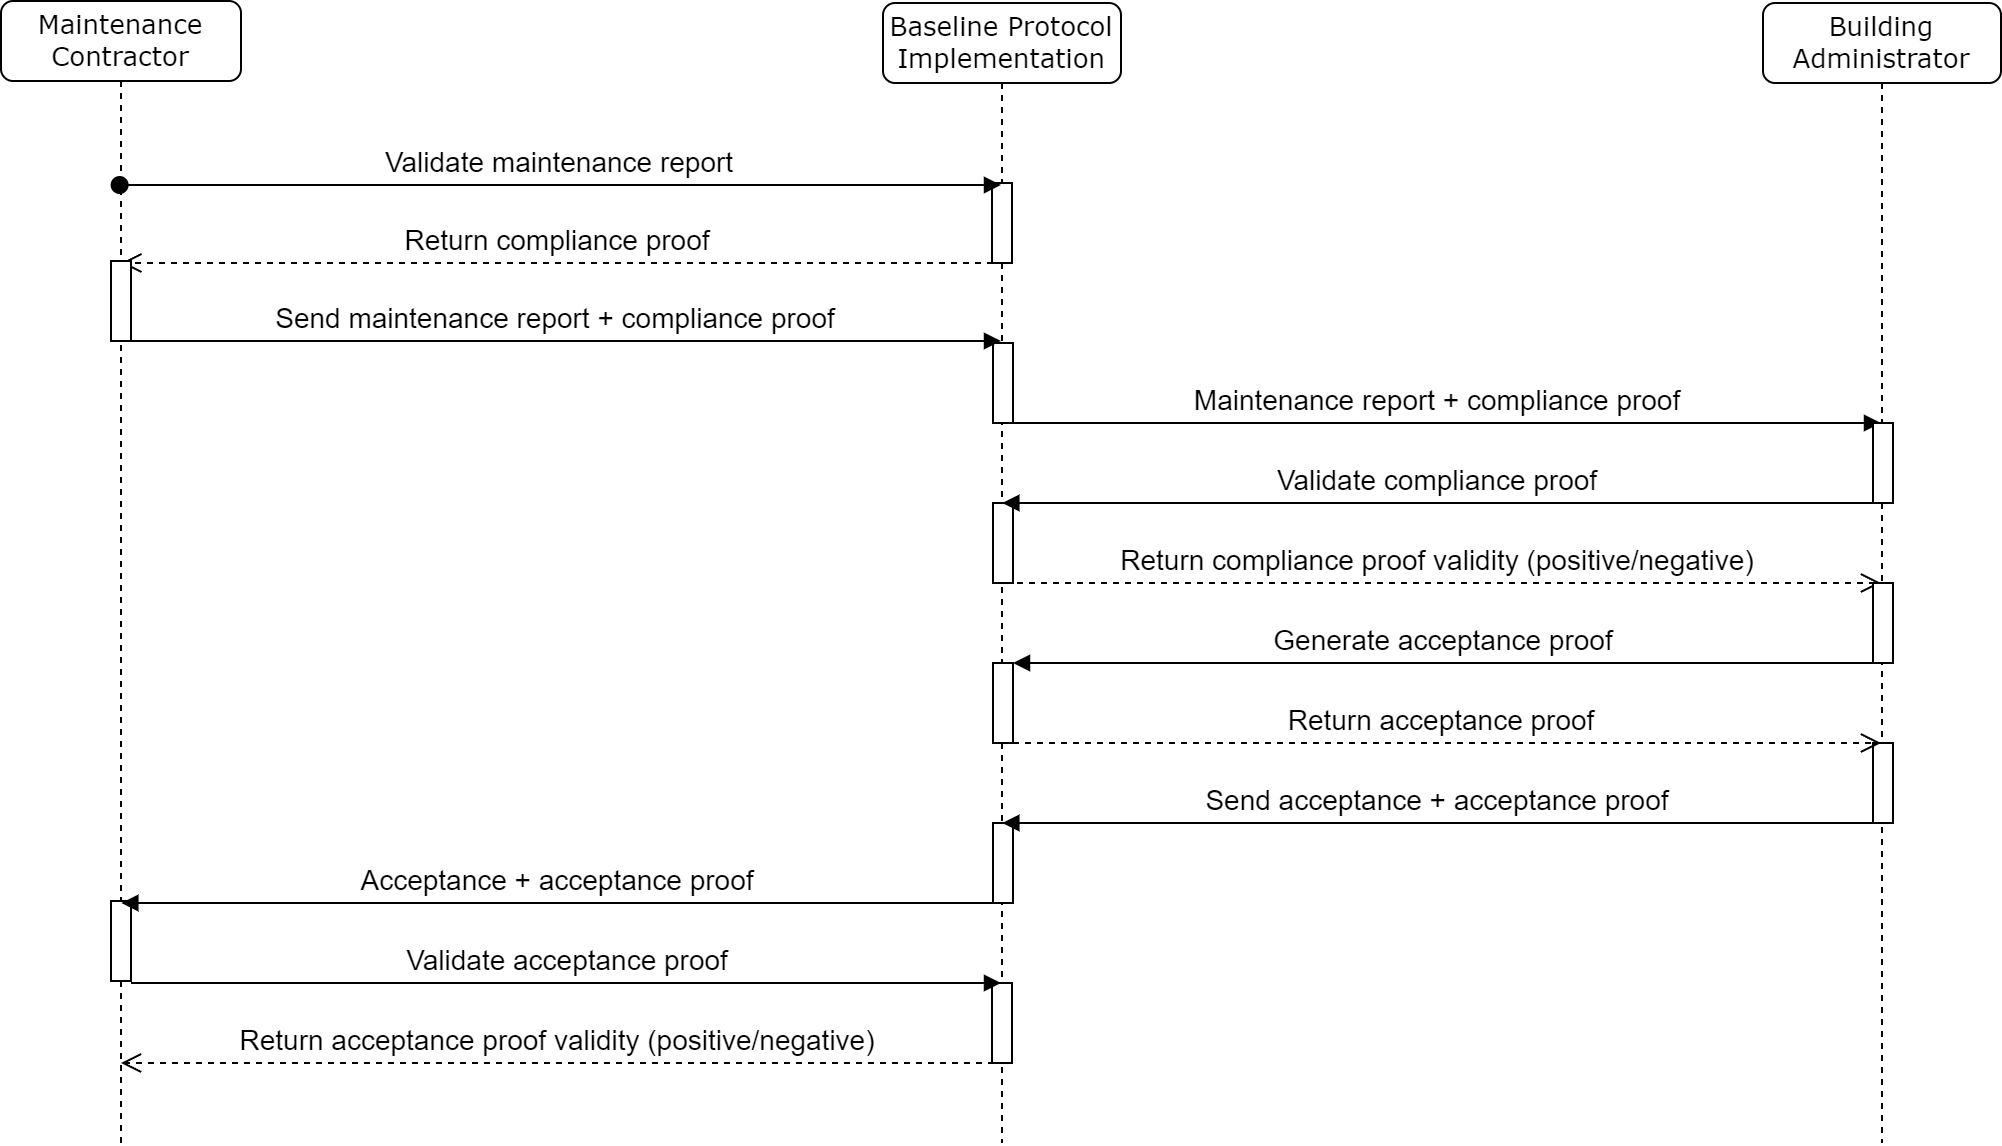
\includegraphics[width=1\textwidth]{background/graphics/maintenance-report-baseline.drawio.png}}
    \caption{Integration of the Baseline Protocol for the exchange of the maintenance report between maintenance contractor and building administrator.}
    \label{fig:background:maintenance_report_baseline}
\end{figure}

After maintenance has been completed, the maintenance contractor sends the maintenance report to the \gls{bpi} API to check its validity. This check is implemented using zero-knowledge circuits\footnote{\glspl{zkp} and ZK circuits are out of scope of this work and will not be further discussed.} that precisely portray the service-level agreements that both parties accepted at the start of the \gls{bp}. If the maintenance report complies, a proof (in the form of zero-knowledge) is returned, and the maintenance report is being transmitted, including the newly generated proof, to the building administrator. Generating proofs, however, is a rather computationally expensive task. Performing it on-chain is therefore unfeasible, considering that hundreds of thousands of proofs must be generated for \glspl{bp} of large companies and organizations. Thus, layer-2 rollup blockchains like Baseledger\footnote{\url{https://baseledger.net/} (accessed on 2022-11-01)} must be employed that are optimized to generate such proofs in a more cost-efficient way. Layer-2 rollups like these, again, only store a \gls{zkp} of the correctness of all \gls{bp} proofs on layer-1 \glspl{ccsm} like Ethereum, to take advantage of the vast amount of participants of such blockchains without exposing any privacy critical data. After receiving the maintenance report with its corresponding compliance proof, the building administrator can now validate the compliance proof to check (1) if the transmitted maintenance report is the one issued by the maintenance contractor and (2) if it is compliant with the previously agreed upon service-level agreement. If the validity check passes, the building administrator can generate a proof that confirms that she accepts the maintenance report in the given form. This proof, once again, can be validated by the other party (in this case, the maintenance contractor)~\cite{baseline_spec}.

Even though the Baseline Protocol is still under heavy development and some of its implementation details are out of scope of this work, given its capabilities, it still holds a lot of potential considering inter-organizational \gls{bpm} and choreographies. Thus, later sections of this work will also investigate possible integrations of the Baseline Protocol into a state machine concept that allows time-traveling verification of \glspl{bp}.
